\section{Introduction}
%<Building Research Partnerships >: Method for Building a Meaningful Disability-Related Research Agenda
%.... Disabilities via their content
%This method bridges close readings from the humanities with technology design related to disability.
In this paper, we explore how online content\footnote{Content and Media are used broadly to mean any created artifact.} created by people with disabilities\footnote{Person-first disability language (e.g., person with disabilities) and identity-first language (e.g., disabled person) are used interchangeably throughout this paper, as is the custom in the communities we worked with.} can be utilized in assistive technology research and design. Empathy building is a common stage of design thinking and human centered design research in which researchers ``set aside their own assumptions'' to get to know user's real needs \cite{plattnerDesignThinkingUnderstand2011,wrightEmpathyExperienceHCI2008}. This stage is used to uncover research questions or design problems. Merriam Webster defines empathy as ``the action of understanding, being aware of, being sensitive to, and vicariously experiencing the feelings, thoughts, and experience of another without having the feelings, thoughts, and experience fully communicated in an objectively explicit manner'' \cite{inc.MeriamWebsterDictionaryDefinition2004}. Empathy has long been considered an important component of participatory design as well as research processes. %Through the empathizing process, designers and researchers spend time getting to know their users and understanding their needs, wants, and objectives.

When used correctly, we believe empathy building can be a powerful first step before beginning participatory design with people with disabilities. A common approach to empathy building is to imagine yourself in someone else's shoes (i.e., what would it be like if I was 10 feet tall?). This approach is not appropriate in the context of learning about people with disabilities. Researchers and designers working with disabled people should be careful to use empathy building to better understand ``being with'' rather than ``being like'' or ``vicariously living through'' users as the definition above suggests \cite{bennettPromiseEmpathyDesign2019}. To be clear, it is not appropriate or effective to do empathy building for people with disabilities though ``trying on'' their disabilities \cite{abreuWhyWonTry2018}.  
We explore how immersing oneself in the content created by disabled individuals can be used to build empathy. It is a way to begin understanding communities before engaging directly with community members during later stages. Taking on this investigation of the community before (but not as a substitute for) working directly with users can be useful for building a basis for appropriate future interactions. 

This could be a small step toward alleviating ``the potential over reliance and under acknowledged use of people with disabilities for their `access labor'...'' \cite{mackWhatWeMean2021,bennettBiographicalPrototypesReimagining2019}. Indeed, methods such as iterative design asks a lot of participants \cite{dourishBeingIteratedAffective2020}.
We encourage researchers to take on some of this initial labor by engaging with and celebrating the pre-existing cultural labor of disabled people \cite{piepzna-samarasinhaCareWorkDreaming2018}. Researchers can build authentic understandings of the needs of populations with disabilities as a precursor to any type of participatory or community-based work without putting undue access work on the community.  

This paper examines how close readings of media produced by people with disabilities can lead to productive empathy building and the discovery of authentic, meaningful research agendas. We propose a nascent method for building this empathy called DREEMing (\underline{D}isability-\underline{R}elated \underline{E}mpathy from \underline{E}xisting \underline{M}edia), which builds on other influential methods from various disciplines described in the Background (Section \ref{Background}), contemporary critiques of the SIGACCESS field discussed in the Motivation (Section \ref{Motivations}), and our own experience of empathy building through three case studies presented in the Case Studies (Section \ref{CaseStudies}). DREEM is a 4-step process that we describe in Section \ref{DREEM}—with actionable tips and insights for how to find appropriate content and develop authentic research agendas. Finally, we discuss DREEMing's novelty, relevance, recommendations for working with research assistants, challenges, limitations, and future work.

In summary, this work builds off of prior research in this space \cite{bennettPromiseEmpathyDesign2019,plattnerDesignThinkingUnderstand2011,wrightEmpathyExperienceHCI2008,shinoharaDesignSocialAccessibility2020} and our primary contributions are a novel 4-step method for building empathy with disabled people via media created by people with disabilities, and materials for using the emreging method, including trainings, data logging templates, and a tool for visualizing close readings. We found that actively engaging with media made by people with disabilities is an opportunity for new researchers to learn about these communities and working with disabled people.

\subsection{Positionality}
We developed DREEM because we are members of the SIGACCESS community and want to design technology that better serves the needs of disabled people. We are inspired by the conversations that took place at previous ASSETS conferences. We are driven to provide actionable insights in \textit{how} we as scholars and academics can do better. DREEM attempts to add a procedure behind these discussions. The team of researchers who developed DREEM work in the <anonymous> Lab focusing on the development of assistive technology at <anonymous> University in the Computational Media department, which is situated in an Engineering environment. The interdisciplinary Computational Media Department bridges engineering perspectives with the Arts and Humanities. Most of the research team are formally educated as engineers, but are familiar with social justice and critical disability studies. At least one member of the team considers themselves as actively engaged in disability justice activism as a member of the disabled community. Our team is made up of people with disabilities and people without disabilities, but each of us is engaged with a population of people with disabilities we are not a part of. We are scholars from varying points in our careers including undergraduates, PhD students, candidates, postdocs, and tenured faculty. We work with a myriad of populations including children with speech impairments, children with physical impairments, autistic people, people with visual impairments, stroke survivors, and people with developmental disabilities.

\section{Background} \label{Background}
 In this section, we begin by discussing the motivations behind DREEM, which include sharing labor with people with disabilities, technosolutionism, contemporary critiques posed to the SIGACCESS community from Disability studies scholars, and documented challenges of employing co-creative, participatory methods with people with disabilities. Next, we discussed the methods and approaches we are inspired by that influenced DREEM.

\subsection{Motivations}\label{Motivations}

A recent survey of ASSETS and CHI accessibility work showed that only 16 methodological contributions (3.2\% of all)  have been made to the accessibility community since 1994  \cite{mackWhatWeMean2021}.
\textbf{What does it mean to create a method that values disabled contributions? } Our guiding principles toward this value are: 
\begin{itemize}
\item  \textit{Labor \ref{Labor}} Honor the work that is already done and value contributor's time. Make disabled contributions meaningful and accessible.
\item \textit{Technosolutionism \ref{Technosoultionism}} Don't come to the table with a solution already in mind. 
\item \textit{Authenticity \ref{authenticity}} Disabled people are not medical patients. 
% \item \textit{Co-Design \ref{cocreationchallenges}} Make disabled contributions meaningful and accessible. Give proper acknowledgment and compensation. 
\end{itemize}

\subsubsection{Labor} \label{Labor}
There are many successful examples of co-creating with disabled people (e.g., \cite{anthonyParticipatoryDesignWorkshop2012,assadMotionBasedGamesParkinson2011,bentonDevelopingIDEASSupporting2012,duvalSpokeItBuildingMobile2018,ellisIncreasingUsabilityOnline2000,ellisParticipatoryDesignInternetbased1998,elorImmersiveVirtualReality2018,karnaDesigningTechnologiesChildren2010,gerlingDesigningMovementbasedPlay2016,grafIGYMInteractiveFloor2019,khaledBridgingSeriousGames2014,malinverniParticipatoryDesignStrategies2014,priorHCIMethodsIncluding2010}). However, we acknowledge the labor required by people with disabilities in both designing and living with existing assistive and accessible technologies. In designing methods that center contributors with disabilities, labor should be carefully considered. A danger of iterative processes, such as participatory design, is how much work we ask of participants who we are trying to help \cite{dourishBeingIteratedAffective2020}. Similarly, access labor refers to the work that people with disabilities are required to do in order to have their access needs met \cite{bennettBiographicalPrototypesReimagining2019,mackWhatWeMean2021,piepzna-samarasinhaCareWorkDreaming2018}. There are concerns such as `informant fatigue' (e.g., being asked too often to share repeated personal details \cite{shinoharaSelfConsciousSelfConfidentDiary2016}) and `forced intimacy' (e.g., being required to divulge deeply private information in order to gain access \cite{mingusForcedIntimacyAbleist2017}). This can also mean maintaining friendly relationships with caregivers \cite{kittayLoveLaborEssays1999}, requesting specific accommodations from event leaders, or the everyday work of living with a disability in an ableist world \cite{hanssonEthicsEnablingTechnology2007a}. We posit that DREEMing ahead of participatory sessions can alleviate the need to use precious time for learning the basics about a population and instead focus on actual co-design work—giving them meaningful ownership as co-designers rather than collecting overly personal information.

The high rates of assistive technology abandonment are due, in part, to the inability of designers to take populations’ perspectives into consideration \cite{gitlinWHYOLDERPEOPLE1995,phillipsPredictorsAssistiveTechnology1993,vandijkEmpoweringPeopleImpairments2016}. Here there can also be a labor cost to using poorly designed technology after it has been developed, as described by many disabled writers (e.g., Forlano \cite{forlanoDangerIntimateAlgorithms2019} or Weise \cite{weiseCommonCyborg2018}). For example, Forlano, a professor of design who sometimes writes about her experience with type one diabetes, must frequently remove herself from meetings and gets woken up in order to recalibrate her automatic insulin pump \cite{forlanoDangerIntimateAlgorithms2019}. If user input has proven to be valuable to designs where the contributions of populations with disabilities are included \cite{karnaDesigningTechnologiesChildren2010,sampleBeginningsParticipatoryAction1996}, why then are many systems designed without leveraging it? Kujala suggests that these challenges stem from arriving to the table with a prototype before doing appropriate ground work \cite{kujalaUserInvolvementReview2003}. Doing groundwork with existing media made by people with disabilities can alleviate many of these concerns for the initial stages of research exploration.

Cultural labor is the organizing and creative work done to contribute to a particular culture such as disability cultures \cite{charltonNothingUsUs2000}. Cultural labor can be in many forms of advocacy including books (e.g., Nothing About Us Without Us \cite{charltonNothingUsUs2000}), legislation (e.g., the Disability Act \cite{civilrightsdivisionAmericansDisabilitiesAct}), or shared accounts (e.g., Resistance and Hope \cite{wongResistanceHopeEssays2018}).  Existing cultural labor is what DREEM relies on. 

\subsubsection{Technosolutionism} \label{Technosoultionism}
Too often, able-bodied scholars wave their techno-magical wands to try and fix problems they believe people with disabilities face \cite{morozovEverythingClickHere2013,charltonNothingUsUs2000}. A prime example of this phenomenon was beautifully articulated by Karen Nakumura during the 2019 ASSETS keynote where Nakumura argued, among other examples, that people who are blind do not want smart white canes because technology dies inconveniently, needs regular charging, is heavy, expensive, and can become a spectacle \cite{nakamuraMyAlgorithmsHave2019}. The white cane is already well designed, so why fix something that already works when there is much real work to be done? Nakumura also posited that if the engineers had simply asked a blind person whether or not they were interested in a smart white cane, they would have quickly moved on. Additionally, a part of this method will be to train undergraduate researchers in the hopes of circumventing some of this thinking early on in their careers \cite{shinoharaDesignSocialAccessibility2020}.

\subsubsection{Authenticity} \label{authenticity}
Over a decade ago, ASSETS scholars called for the use of a critical disability lens while designing and developing assistive technology for disabled individuals \cite{mankoffDisabilityStudiesSource2010}. This call has only strengthened in the proceeding years, with an emphasis on allowing for more co-design and co-research with disabled people \cite{bennettPromiseEmpathyDesign2019,ymousAmJustTerrified2020,spielAgencyAutisticChildren2019}. To summarize the concern, the majority of assistive technology devices and applications are rooted in medical discourse. That is, disability is an inherent problem in the body and must be ``fixed'' or ``normalized'' by intervention. Using a more socially-oriented lens, such as those found in disability studies, emphasizes the social context and environment as \textit{creating} disability by denying access to particular body configurations \cite{ginsburgDisabilityWorlds2013,ringlandPlacePlayDis2019,titchkoskyQuestionAccessDisability2011}. There is also an ongoing conversation in disability studies works that examine disability as a culture and identity \cite{kaferFeministQueerCrip2013}, which also leads to a re-examining for those designing assistive technology of the \textit{purpose} of that technology. Given this concern about the discourses that influence the design of assistive technologies, it has become even more important for researchers to acknowledge the needs of the disabled individuals the technology is meant to help. DREEMing can potentially offer a lens into the sociocultural fabrics of disabled communities.

%\subsubsection{Co-Creation and Participatory Design Challenges with People with Disabilities} \label{cocreationchallenges}
%There are many successful examples of co-creating with disabled people (e.g., \cite{anthonyParticipatoryDesignWorkshop2012,assadMotionBasedGamesParkinson2011,bentonDevelopingIDEASSupporting2012,duvalSpokeItBuildingMobile2018,ellisIncreasingUsabilityOnline2000,ellisParticipatoryDesignInternetbased1998,elorImmersiveVirtualReality2018,karnaDesigningTechnologiesChildren2010,gerlingDesigningMovementbasedPlay2016,grafIGYMInteractiveFloor2019,khaledBridgingSeriousGames2014,malinverniParticipatoryDesignStrategies2014,priorHCIMethodsIncluding2010}), which we discuss in Section \ref{PD}, but there are also many documented and pragmatic challenges \cite{wardReflectionsParticipatoryAction2001}. The high rates of assistive technology abandonment are due, in part, to the inability to take populations’ perspectives into consideration \cite{gitlinWHYOLDERPEOPLE1995,phillipsPredictorsAssistiveTechnology1993,vandijkEmpoweringPeopleImpairments2016}. If user input has proven to be valuable to designs where the contributions of populations with disabilities are included \cite{karnaDesigningTechnologiesChildren2010,sampleBeginningsParticipatoryAction1996}, why then are many systems designed without leveraging it? Documented obstacles to implementing participatory design include identifying users, obtaining access to users, motivating co-designers, ineffective feedback strategies, time constraints, issues identifying consensus, limited design competencies, overwhelming amounts of data, difficult scheduling logistics, and costs of developing changes \cite{kujalaUserInvolvementReview2003}. We believe many of these challenges can be alleviated with more preparation and empathy—often our assumptions and inaccessible protocols are the root of the issue, not disability. Kujala suggests that these challenges stem from arriving to the table with a prototype before doing appropriate ground work \cite{kujalaUserInvolvementReview2003}, similar to our technosolutionism arguments above. Doing groundwork with existing media made by people with disabilities can alleviate many of these concerns for the initial stages of research exploration. 

%Co-Design sessions should be valuable to all parties \cite{bodkerParticipatoryDesignThat2018}, especially as they disrupt everyday life and require participants to invest their precious time. We again nod to issues of labor in participatory design with people with disabilities. `Informant fatigue' happens when disabled people (usually those with visible disabilities) are too often asked to share details about their disability with others who ask \cite{shinoharaSelfConsciousSelfConfidentDiary2016}. This can also take the form of `forced intimacy', where a disabled person has to divulge what would normally be highly personal information in order to have their access needs met in a given context \cite{mingusForcedIntimacyAbleist2017}. Both informant fatigue and forced intimacy can occur in design research with people with disabilities if researchers are not careful. Work remains to be done in centering disabled people as designers for the contributions that they make \cite{bennettBiographicalPrototypesReimagining2019} and for compensating co-designers appropriately. We posit that DREEMing ahead of participatory sessions can alleviate the need to use precious time for learning the basics about a population and instead focus on actual co-design work -- giving them meaningful ownership as co-designers rather than collecting overly personal information.

\subsubsection{Novelty}
As discussed above, there has been much discourse on how the SIGACCESS community needs to do better in regards to technosolutionism, authenticity, and inclusive design, but to our knowledge there has not been actionable processes towards addressing these issues. DREEM is a bridge between contemporary critiques and actionable steps towards building research agendas that will support a more inclusive and accessible society. DREEM is intended to support new scholars and those interested in contributing to the SIGACCESS field.
			
\subsection{Influential Methods and Approaches}\label{influences}
As mentioned in Section \ref{Motivations}, there are relatively few methodologies designed specifically for use by the SIGACCESS community. Accessibility research draws on existing research methods such as those from human computer interaction, computer science, design, psychology, and sociology. In this section we discuss the multidisciplinary methodologies that informed the creation of DREEM. 

\subsubsection{Close Readings\label{CloseReadings}}
Close readings are the careful, deliberate observation of an artifact \cite{brummettTechniquesCloseReading2019}. Close reading is about \textit{seeing} what is there (and not there). It is about mindfulness, noticing, and reflection \cite{brummettTechniquesCloseReading2019}. Close readings afford the wandering mind to ask questions about what is and is not present and reflect on the possibilities in a larger context. The method originated in literary studies, and is typically conducted on text. Close readings can also be applied to other designed artifacts such as games (e.g., \cite{wardrip-fruinHowPacManEats2020}), software (e.g., \cite{sackSoftwareArts2019}), videos, film, and images. Close readings are typically conducted by scholars in the humanities, but there is potential for designers to leverage close readings more broadly. If a close reading is the mindful, disciplined reading of an object with a view to deeper understanding of its meanings \cite{brummettTechniquesCloseReading2019}, then it has the potential to help us understand the experience of living with a disability more deeply. In short, close readings can help us build empathy. DREEMing relies on close readings and provides suggestions on how to find relevant media.

\subsubsection{Netnography}
Netnography is an online research method originating in ethnography and is often employed by social scientists and anthropologists \cite{kozinetsNetnographyEssentialGuide2019}. Instead of focusing on typical embodied phenomena in ethnography such as body language, netnography focuses primarily on the context of online media such as text and multimedia \cite{bartlReviewAnalysisLiterature2016}. Netnography is typically conducted on a smaller scale than sentiment analysis run on large data sets and provides more nuanced behavioral findings than automated software. Netnography is a subset of digital ethnography, with netnography focusing more on the individual encounters across social media.  Since Netnography uses spontaneous data and conducts observation without intruding online users, it is regarded as more naturalistic than other approaches such as interviews, focus groups, surveys and experiments \cite{kozinetsNetnographyRedefined2015}. These online community members often share in-depth insights on themselves, their lifestyles, and the reasons behind the choices they make \cite{kozinetsNetnographyEssentialGuide2019}.  For DREEM, these communities are populations with disabilities and the media discovered provides a basis to conduct a close reading for empathy building.

\subsubsection{Situated Play Design}
Situated Play Design (SPD) is an open methodological framework for surfacing existing manifestations of play in everyday life to inspire technology design \cite{altarribabertranChasingPlayPotentials2019a,altarribabertranDesigningPlayThat2019}. SPD has been used on TikTok to find playful content from creators with disabilities to inspire playful everyday technology (not necessarily assistive technology) \cite{duvalChasingPlayTikTok2021}. The 3-step approach outlined in SPD served as a model for us in finding online content for contextual technology design. DREEM differs from SPD in that we are not focused on play in this work and instead of directly inspiring technology design, DREEM is focused on developing research agendas. Similar to SPD, we view DREEM as a Research Through Design project itself \cite{gaverWhatShouldWe2012,zimmermanResearchDesignMethod2007}—an open methodological framework that can be adapted and improved through community contributions. 

\subsubsection{User-centered Design and Participatory Design} \label{PD}
These related design approaches strongly emphasize a need for user involvement in all stages of design.
From exergames for wheelchair users \cite{gerlingDesigningMovementbasedPlay2016} to speech therapy \cite{duvalSpokeItCoCreatedSpeech2018}, virtual reality for teaching people with developmental disabilities to identify emotions in others  \cite{thangPhDForumStrengthening2018}, and robots for physical rehabilitation \cite{marquezseguraPlayificationPhySeEarCase2016}, technology can effectively be designed with and for people with disabilities. For facing the next generation of big issues that matter, all stakeholders should participate in the design of technology they will use \cite{bodkerParticipatoryDesignThat2018}. DREEM fits within the larger umbrella of participatory methods by leveraging existing cultural work to educate researchers prior to co-design sessions so that they can be more effective and appropriate. DREEM is not a replacement for participatory work, it is a precursor.

\subsubsection{Autoethnography}
Autoethnography is a type of ethnographic work that is conducted of one's own experiences and contexts. ``Autoethnography is a theoretical, methodological, and (primarily) textual approach that seeks to experience, reflect on, and represent through evocation the relationship among self and culture, individual and collective experience, and identity politics and appeals for social justice'' \cite{holmanjonesAutoethnography2007}. The results of autoethnography then ''represent [the autoethnographer's] thoughts, emotions, collective experiences, and social processes associated with an identity or issue and then contextualize them in broader, societal‐level phenomena'' \cite{ramboAutoethnography2020}. This approach may employ a standard written essay format, a diary log, or handwritten annotations as well as more artful forms such as plays, art, music, and poetry. Autoethnography is an appropriate reflective practice while conducting close readings to develop empathy. DREEM pairs close readings with autoethnography to generate the appropriate type of empathy that can make participatory work more productive and appropriate.

\subsubsection{Inductive Thematic Coding}
Thematic analysis allows researchers to explore themes (overarching categories of common data) with the aim of  understanding emerging phenomena that appears and communicate findings with other researchers \cite{guestAppliedThematicAnalysis2012}. Inductive coding is especially relevant for the creation of new research agendas because it allows us to find novel areas, problems, and gaps to focus on. Inductive thematic coding is relevant to DREEM because it offers a grounded and established basis for generating research questions and communicating findings.

\section{Method}
The research questions that inspired the development of DREEM and this paper are: 
\begin{enumerate}[label=RQ\arabic*:]
% \item \textit{How can the SIGACCESS community develop research agendas that are genuine to the needs of people with disabilities through appropriate empathy building?}
\item \textit{How can assistive technology researchers and designers utilize media made by disabled people in their work? (DREEM)}
\item \textit{What types of insights does DREEM offer?} %through employing it in case studies?}
\item \textit{How can scholars adopt DREEMing efficiently?}
\end{enumerate}

% For \textit{RQ1}, we conducted a comprehensive literature review presented in the background section that includes motivations and influential works that drove the development of DREEMing. 
For \textit{RQ1}, we experimented with a methodological framework which we call DREEM (\underline{D}isability-\underline{R}elated \underline{E}mpathy from \underline{E}xisting \underline{M}edia). The process, motivations, and results of developing the DREEM framework are detailed herein. 
\textit{RQ2} is related to the \textit{value} of DREEM, which we illustrate through our case studies. We use this section to describe how we conducted DREEMing with team of researchers towards iterating on the method itself and building the case studies. For \textit{RQ3}, we use autoethnographic reflections presented in the discussion section to share the insights, limitations, and value of DREEMing. 

To develop the DREEM framework we began with these 3 steps:
\begin{enumerate}
\item Discover Existing Media
\item Close Reading
\item Autoethnographic Reflections
\end{enumerate}

%To evaluate the effectiveness of DREEMing, develop tools to assist with its implementation, and develop insights on its future and limitations (\textit{RQ2}), 
We took a research through design approach \cite{gaverWhatShouldWe2012, zimmermanResearchDesignMethod2007} and employed DREEM while iterating on its implementation through three case studies which we present in the following section. In this section, we describe the process of employing DREEM with four undergraduate research assistants. In the following sections, we discuss its final evolution.

Prior to recruiting undergraduate research assistants, the senior research team, who designed the initial version of DREEM, completed steps 2 and 3 on \textit{The Power of Choice} (\url{https://www.youtube.com/watch?v=B1sWtT-wShI}) independently. Afterward, we collaborated on tweaks to the data collection process and included our findings as a case study in the training materials we developed. We recruited four RAs through department news letters and by advertising in classes we teach. Our research flier is included in an editable form in our supplementary materials at \url{https://tinyurl.com/DREEMRecruitment}. We accepted all applications. We then used \textit{When2Meet} to find a time everyone was available for a on-boarding training session. The hour-long training described the motivations of the work, instructions on how to carry out the work, and expectations. An editable version of our training slides are available in the supplementary materials at \url{https://tinyurl.com/DREEMTraining}. We asked undergraduates to reflect on their interest and confirm whether or not they wanted to participate as a collaborator. RAs then used our DREEM form (available in the supplementary materials as an editable google form at \url{https://tinyurl.com/DREEMForm}) to independently and asynchronously conduct steps 1-3. We had a reoccurring weekly check in where we  discussed progress, research directions, and reflections as a team. Our specific case  studies were born from exploration and interest-driven directions lead by the RAs. After 3 weeks, interns participated in the inductive data analysis and helped us construct the write-up for the case studies presented in this paper.

\subsection{Ethics}\label{Ethics}
A tricky element of our research is discovering existing content on social media and the ethical implications of researching on these platforms. Our data collection method closely aligns with \textit{Netnography} \cite{kozinetsNetnographyEssentialGuide2019}, which has established ethical guidelines \cite{kozinetsEthics2019}. These include the notion of public versus private information on social media, whether to anonymize or cite participants, and informed consent. Kozinets argues that ethical procedures must be decided on a case-by-case basis contingent upon the topic matter, the research purposes and the research approach of the particular \textit{netnography} \cite{kozinetsNetnographyEssentialGuide2019}. Some platforms such as Facebook and Instagram have varying levels of security and privacy settings for content and profiles that complicate what is truly public. Researchers using platforms with privacy settings must respect what is considered public and not. Bassett and Kozinets argue that when the internet is used as a ``megaphone-like'' public broadcasting medium \cite{mcquarrieMegaphoneEffectTaste2013}, we can thus perceive it as a form of cultural production, in a similar framework to that of the print media, broadcast television and radio where we should cite the source so that broadcasters can be credited for their work \cite{bassettEthicsInternetResearch2002,kozinetsEthics2019}. Sometimes content posted online is ephemeral such as temporarily available stories. To respect creators wishes, we did not include these media in our case studies. Because this research is minimal risk and fits the notion of public broadcasting online, we provided links to the original content in our published materials to respect the creators' (ongoing) decisions concerning public access to the videos. \textit{Netnography} of public archival content (not active research interventions such as interviewing) such as the media discovery methodology employed in this research would be unduly complicated with informed consent because the manual, non-automated access by researchers of public information should be acceptable without special permissions or actions \cite{allenAcademicDataCollection2006} and removing information from unreachable broadcasters would undermine researchers' ability to contribute to society \cite{kozinetsEthics2019}. Therefore, we included all applicable data scraped in our supplementary materials and make every effort to represent the content in this publication respectfully and in a positive light. Finally, our data was manually discovered without any automated system or software and is not used for commercial purposes, and therefore, at the time of writing to the best of our knowledge, adheres to the terms of services of these platforms.

\section{Case Studies and Value} \label{CaseStudies}
In this section we present three exploratory case studies which use the DREEM framework. 
We then present a survey of researcher learnings from conducting these case studies. 
All authors contributed to close readings for the case studies, but the quotes within this section are anonymized.

 Research team collaborators were free to explore any media form of interest, platforms, and communities—as long as the content was created by a disabled person. After an inductive analysis, the close readings and reflections were sorted into 8 emerging non-mutually exclusive themes: ableism, aesthetics of personal expression, autism, traveling with a vision impairment, everyday tasks with a vision impairment, tourettes, mobility, and communication, which are all available in the supplementary materials at \url{https://tinyurl.com/DREEMData}. We chose to present 3 in this paper to evaluate our initial version of the DREEM method including: ableism, tourettes, and Beauty Products and Aesthetics. 

\subsection{Case Study: Ableism} \label{case:ableism}
In this case study, three researchers close read five media sources around the topic of ``ableism.'' Two of those sources were text-based articles, one TikTok video, and two YouTube videos. Each of these media were addressing and describing different aspects of ableism encountered by the creators. The content ranged from educational to emotional and personal.

The first article described the author's experiences during a year of lockdown due to the COVID-19 pandemic. The second article described the experiences of disability in a hospital setting. Both addressed issues of ableism towards them as a result of disability and the impact of that ableism on their respective experiences. It is worth noting that for the second article, the researcher was unable to finish the close read as it was ``really emotional'' and, therefore, they chose to put it away for the time being. We will come back to discussing the difficulty in doing this type of analysis in the Discussion (Section \ref{Discussion}). 

The YouTube videos were longer-form content that was more educational and explanatory in nature. One was about traveling in Paris with disability and the other was a video log (vlog) educating about ableism. The third video was on TikTok, and therefore only one minute long, and was a personal description of how a student had experienced discrimination for both their gender and disability from their math professor.

For these five media, three had completed autoethnographic reflections. All three reflections were about the researcher's epiphanies and new understandings about disability and ableism after having close read the media. For example, one researcher wrote, ``[a]bleism and other discrimination could stem from the lack of education.'' Another researcher wrote, ``systemic Ableism does not disappear even when top officials try to implement a fair approach.''

The close reading of content about ableism allowed the researchers to analyze and reflect on information about discrimination of disabled people first hand. For example, in the video about the student experiencing discrimination from their professor, the researcher reflected on the situation and asked some rhetorical questions in their close reading. For this researcher, they reflected on the use of particular language by the creator,
\begin{quote}
    ``The professor responses and belittles the creator whenever they make a make a mistake or a question. The creator also relates this situation to being treated a like a child. Do they make this comparison because they feel like they are smaller or helpless? There are other ways to describe being condescended or put down, and them deciding to compare to how a child is treated by an adult is interesting.''
\end{quote}
While discourse around those with disabilities being treated like children is common in disability communities, this was something new for the researcher doing the close reading. Later in the same video, the researcher comments in their close read, 
\begin{quote}
    ``It seems ironic that this school has an Office of Disabilities, and yet this professor still acts this way, which points to the fact that the office has not yet action for this professor's behavior. Has no student or other staff reported the professor? I wonder why.''
\end{quote}
In this one minute TikTok video, the researcher has come upon a number of different effects of systemic ableism. Future research in this direction would most likely uncover more of this type of findings. Doing this close reading first before approaching members of the disable community allows this researcher to begin to have an understanding of some of the barriers that those with disabilities face.


\subsection{Case Study: Tourette's Syndrome Case Study}
We chose to include this case study because it offers an interesting perspective on how the affordances of various social media platforms can affect the types of insights DREEMing can offer. 65 out of 70 of the close readings and autoethnographic reflections related to tourettes across 7 media sources were completed by 1 highly motivated undergraduate researcher. The media sources include a personal website (hosting a blog, \textit{Youtube} videos, tweets, and a shop promoting Tourette's awareness), 5 \textit{YouTube} Videos, and 3 TikToks. 

The first media source is a personal website, called \textit{TicTastic!}, written by a 14 year old musician who attends school, surfs, blogs, bakes, and has Tourette's syndrome and Obsessive Compulsive Disorder. Close reading a website that hosts a variety of media surrounding 1 individual's perspective offered a depth that was unique to our learning.
\begin{quote}
Seeing a new and darker side of her experience made me realize and remember that not all publicity/media coverages will correctly and fully represent a disability (or anything really).
\end{quote}
This question of \textit{true} representation of media coverage is interesting—and we were particularly puzzled by some media on \textit{TikTok}. While there were sources of wholesome media on TikTok related to tourettes (e.g., a couple playfully forgiving each other after a tic caused accidental physical contact), there was also videos that made us ponder the disabled creator's intent. For example, one creator created a highlight reel of their tics while cooking pasta and many of the comments seemed offensive—why did the creator post this? Was it for comedic relief, authentic lived experience, visibility, or something else all together? Unanswered questions are why DREEMing can promote empathy and foster new partnerships. 

\textit{TikTok's} short videos offer quick flashes of insight—whether they are rants, humorous moments, or viral challenges—but they often leave use with more questions than answers, which is not counterproductive. \textit{Youtube} on the other hand, affords much longer videos and more content, but the general population may be less inclined to spend their time watching a longer \textit{YouTube} video as compared to the negligible time it takes to watch 1 \textit{TikTok}. In a reflection by one of the researchers discovering content on \textit{YouTube}, they were surprised at the patience of the content creator's friends and family:
\begin{quote}
It was great to see the positive reactions in the moments of accidents, and that showed that these people understood how and why tics happen. And it seems to remind the importance of education and how that allows people to empathize and understand. It also makes me think that educating people on disabilities would help to create a better environment and society without ableism. 
\end{quote}
\textit{YouTube} was also an effective platform for us to discover subgroups of the tourettes community—particularly those who are also gamers. One of the videos showed a woman playing the popular game, \textit{Among Us}, a multiplayer mobile game where players finish tasks on a spaceship while impostors try to eliminate the crew mates and players try to deceive each other in an interactive \textit{whodunit}. The researcher reflected on the possible effectiveness of using games as a platform for increasing disability visibility and education. When using DREEM on various platforms, it is important to consider each platform's affordances as well as who the intended audience the content was made for (e.g., a video for fellow members of a disabled community or a video for the general public). 

\subsection{Beauty Products and Aesthetics}
We chose to include this case study because it is agnostic of disability, but instead discusses a specific topic. For this case study, two researchers considered three sources. Two of those sources were videos, the third was a makeup line release. The makeup line release was "Rare" by Selena Gomez. Selena Gomez has Rheumatoid Arthritis. The makeup line features products with spherical lids that allow a user to push down instead of squeezing to open. 

The first video was a product review by Molly Burke, a YouTuber and makeup enthusiast who is blind. Through Burke's video we learned the importance of organization, scent, and embossing are for her in any makeup palette. One researcher reflects on the impact of packaging in accessible design for makeups:
\begin{quote}
    Watching this video taught me to focus more on the small but impactful details on makeup products that affect one’s ability to utilize it effectively
\end{quote}

Burke calls out large makeup companies for not having inclusive design. We think more people with disabilities should be making design decisions in the beauty industry—just like Selena Gomez's new line. 

The second video is on a morning routine for particularly anxious days made by Asia Jackson. Our main takeaway from this video was that jewelry and fashion can be used to ritualize self care. Putting on your favorite jewelry before beginning a process you may otherwise struggle with can make it more approachable and fun. Fashion can be used in many empowering ways, even if no one but yourself can see it. It is important that fashion is accessible in general and for the purposes of self-empowerment.

We would like to explore further how technology is already used and could be used for product recommendations by people with disabilities. People with different disabilities will likely have different product needs. For example, scent would be a barrier to people with chemical sensitivities, but Burke benefits from Too-Faced's food scented products. Further, we would like to explore how these recommendations from people with disabilities could help companies do better. 

\subsection{Researcher Learning Survey}\label{survey}
As we explored what could be learned from existing media with the undergraduate team, we discovered one of the primary contributions of the paper: Actively engaging with media made by people with disabilities can be an effective way for new researchers to learn about communities and working with disabled people. Each of the four undergraduate researchers had never previously conducted assistive technology research. 

We anonymously surveyed the team after they participated in creating the case studies above. The survey consisted of both an adaptation of the Teach Access survey made by the Ability Project \cite{kearney-volpeEvaluatingInstructorStrategy2019}, and the Multidimensional Attitudes Scale Toward Persons With Disabilities (MAS) \cite{findlerMultidimensionalAttitudesScale2007}. We also added questions on the perceived usefulness of the exercise. The only adaptation from the Teach Access survey was dropping the question on Web Content Accessibility Guidelines due to lack of relevance. 

MAS delivers a vignette about a person (Joseph/Michelle) waiting with a friend of a friend who is a wheelchair user. The survey consists of 34 items rated on a 5 point Likert scale. The 34 items are categorized into three sub-domains: cognition, affect, and behavior. Users are asked to rate the likelihood that Joseph/Michelle experiences the 34 cognitions, affects, or behaviors. Scores are calculated by taking the average of all responses within the three sub domains, where scoring lower is better. The undergraduate team N(4) scored an average of 2.36 for cognition, 2.85 for affect, and 2.56 for behavior.  

The Teach Access survey consists of 11 items (which we reduced to 10) rated on a 5 point Likert scale. The first 8 items (reduced to 7) are self-reports of confidence in understanding of accessibility concepts. The last 3 are self-reports on interest in pursing accessibility related work. The average response to each question is illustrated in Table \ref{tab:survey}. It is no surprise that the team is highly interested in pursuing accessibility related work (Q 8-10) as they self selected into this research project. 

\begin{table*}
  \caption{Teach Access Survey}
  \label{tab:survey}
  \begin{tabular}{clc}
    \toprule
    Q&On a scale of 1 to 5, how confident are you that you could do each of the following at this time?&Result\\
    \midrule
    1 & Give an example of a type of disability& 5\\
    2 & Define‚ Accessibility as the term relates to technology and media & 4.5\\
    3 & Give an example of inclusive or universal design & 4\\
    4 & Give an example of how accessible technology is used by people with disabilities& 4.5\\
    5 & Give an example of how assistive technology is used by people with disabilities & 4.25 \\
    6 & Give an example of a technological barrier somebody with a disability might face & 4.25 \\
    7 & Define the purpose of the Americans with Disabilities Act & 2.75 \\ 
    8 & Learning more about designing or developing technologies for and with people with disabilities & 4.5 \\ 
    9 & Pursuing a job or career in accessible technology & 4.25 \\ 
    10 & Pursuing research in the development of accessible technologies. & 4.5 \\
  \bottomrule
 
\end{tabular}
\end{table*}

In addition to the measures above, we asked the team to report on if and how DREEM has changed their perspectives, whether it was a good use of time for the effort, what was most difficult about it, and what impact (if any) DREEMing had on their knowledge of disability best practices. Researchers report better understandings of potentially ableist actions: 
\begin{quote}
    "As an abled person, I understand better the importance of including into any conversation instead of trying to speak for [disabled people]"
\end{quote}

The team found value in their readings: 
\begin{quote}
    "Instead of just doomscrolling or just scrolling in general, it gives me a focused reason to open social media and experiment with its algorithms to find communities I wouldn't normally find myself in. I feel that it's a good way to resist the algorithms that naturally filter us into niches."
\end{quote}

And that there's still work to be done for access: 
\begin{quote}
    "[DREEMing] taught me certain aspects of accessibility, especially in the beauty industry, are still not accessible to most people with disabilities"
\end{quote}
  
All researchers report writing "thoughtful comments" being the most difficult part of the close reading process. As one researcher puts it "I kept on double thinking myself about whether or not I was properly empathizing with the subject's needs"

As a whole, one researcher thinks DREEMing think more broadly about disabled people's experiences:
\begin{quote}
        "Rather than changing my attitude, DREEM helped to broaden my perspective and taught me to look beyond what is portrayed."
\end{quote}
  

% Quotes to add: 
% Perspectives: 

% "As an abled person, I understand better the importance of including into any conversation instead of trying to speak for them."

% "Rather than changing my attitude, DREEM helped to broaden my perspective and taught me to look beyond what is portrayed."

% "it has broadened my vocabulary to be able to talk more colloquially about disabilities. For instance, the word "stimming" in relation to ASD and ADHD"

% Use of time

% "Yes! Instead of just doomscrolling or just scrolling in general, it gives me a focused reason to open social media and experiment with its algorithms to find communities I wouldn't normally find myself in. I feel that it's a good way to resist the algorithms that naturally filter us into niches."

% Impact 
% "This method taught me certain aspects of accessibility, especially in the beauty industry, that are still not accessible to most people with disabilities"

% "To not assume things in a way that enables ableism and actually communicate, ask questions, and collect their input. As someone who wants to work in tech, coming across the concept of ethical design is something I will bring with me. "

% "It showed me how important testing, or at least being able to have a disabled consultant while designing products is. ... a lot of disabled people generally have good ideas as to what [tech] they need [to be made]...It also showed me how important modular/customizable design is, since disabilities affect each person differently."

% Difficulties: 
% "Writing thoughtful comments about a timestamp"
% "Sticking to annotations and not doing summaries"
% "I just kept questioning myself if the comments/analysis that I was writing was good enough."
% "I kept on double thinking myself about whether or not I was properly empathizing with the subject's needs and I couldn't determine if there was a proper way of empathizing with a person."


  
\section{DREEM} \label{DREEM}
In this section, we introduce the 4 resulting steps to DREEMing. The process of completing this methodological framework is inspired by the influences discussed in the previous sections. Each of the four steps are discussed in detail with tips and insights derived from employing the method in the case studies described in the following section (Section \ref{CaseStudies}). The nature of DREEMing is qualitative and, therefore, a quantitative evaluation of the method is not appropriate (at least until more case studies adopt the method, when a systematic analysis can be conducted). Instead, we illustrate the value of DREEMing through the contributions of three case studies and through the autoethnographic reflections \cite{ramboAutoethnography2020} in our Discussion (Section \ref{Discussion}). Steps 1-3 can be repeated for as long as necessary until data saturation is reached. For data saturation, we recommend using a diverse range of platforms, media mediums, and finding numerous subgroups within the target community.  It is possible that steps 1-3 will need to be revisited and repeated based on later research phases. 

After reflecting on our case studies and survey of the researchers, in addition to our original three steps of the DREEM process, we have added a Step 4 (Generation of Research Agenda). This step allows the researcher to reflect on their findings and refine them into a potential path forward for the research.

Below we offer a detailed explanation of each step of DREEM along with our insights based on our experiences employing a version of the method. In each step, we pose some ``tips for success'' that we generated after our own stumbles in using and training in DREEMing. We conclude this section with suggestions for presenting the findings from DREEM and our reflections on DREEMing as a team.

\subsection{Step 1: Discovering Relevant Media}
We consider any public medium to be of potential for DREEMing including blogs, images, videos, films, tweets, and posts. So far, we have primarily considered videos and text-based pieces in our case studies. Mediums such as visual art are certainly possible, but require further exploration and a grounding in visual studies.  We focus on media that can be found online for ease of access. There does, of course, exist important media made by people with disabilities that cannot be found online. It is possible to close read in-person performances, but having a recorded version offers the ability to sit with and return to the content. Zines and event ephemera could also offer interesting insights. This method could reasonably be extended to any of the above (and more!).

\subsubsection{Tips for Success}
Finding media created by people with disabilities online can be a surprisingly difficult task. For example, when looking for content from creators with autism, searching for ``autistic'' might seem like a good place to start. Unfortunately, it will likely result in informational content such as the biology of a disability rather than the lived experience or perspectives from a non-disabled creator. Furthermore, finding such media may require some prior community knowledge (hashtags, vocabulary, etc.) that may be difficult to access for an outsider. We found that trying to find ways ``in'' to a community via hashtags or through snowball methods were the easiest way to find appropriate content. We offer the following tips for success in finding content creators with disabilities online. Examples of each are listed with each tip. 
 
\begin{itemize}
  \item Search common content with flavor: `what's in my bag: chronic illness edition', `amputee morning routine'
  \item Learn community hashtags and keywords, which vary from platform to platform: \#ActuallyAutistic, \#Spoonie, \#CripTheVote, \#ADHDTwitter
  \item Train the curation algorithm: Create a new social media account and follow only creators with hearing impairments as you find them. 
  \item Snowball: Discover accounts that a creator you follow tags. 
  \item Look for collectives and anthologies: SinsInvalid, Disability Visibility Project
\end{itemize}

% \subsubsection{Potential Pitfalls}
% Media found may not perfectly represent the community as a whole. Here are several pitfalls to consider when finding media. Things to look out for include any media that perpetuates ableism, only exposing yourself to a small subgroup of a larger community, and anything that has been shared exclusively with a private network (See Section \ref{Ethics}). 

\subsubsection{Important Considerations}
There are several pitfalls to finding media on the web. We encourage DREEMers to carefully consider whether certain media sources need to be taken with a grain of salt, supplemented, or left out all together. First, consider whether the media source perpetuates ableism and how. If you do not feel confident in detecting ableism, or could use a primer, you might first consider seeking out media made by disabled people on how ableism appears. A good place to start might be with some of the videos discussed in Section \ref{case:ableism}. Second, media is not all-telling. It is made by individuals or small groups, and may not represent the community as a whole. It is important to explore different perspectives from creators with disabilities. Third, anything that has been shared exclusively with a private network should probably be kept that way (See Section \ref{Ethics}). Fourth, different social media platforms have different affordances and cultures. A TikTok video may be curated for a specific ``in-crowd'' audience because of the nature of community building inside the platform, while a YouTube video might be for a broader audience because of its longer-form and reach. Last, relatedly, consider who the target audience is for the source. It is highly possible that the media wasn't made for outsiders to the community and uses terminology or makes light of certain subjects that would not be appropriate for an outsider.

\subsection{Step 2: Close Reading}
This step requires reading or observing the media, and sitting thoughtfully with it as described in Section \ref{CloseReadings}. We recommend working systematically and using standardized collection measures. We include an editable Google form for DREEMing in the supplemental materials at \url{https://tinyurl.com/DREEMForm}. Relevant details to log beyond the close reading itself include the source of the media, a short 1-5 word summary that makes skimming the data later easier, annotated screenshot(s), location in the media the close reading entry relates to (e.g., line number, time span in video), and keywords/tags. We enter each ``complete thought'' as one unit—these could be a few words or a few sentences. We also logged questions we asked ourselves that arose during the close readings. You can choose to immediately start logging your visceral reactions or start entering close readings after you've been fully exposed to the media, but we recommend doing both.

\subsubsection{Tips for Success}
Record your thoughts as they occur. These can directly relate to the content in the video or can be personal to your lived experiences. As you go, maintain a list of keywords and tag each recorded thought. These keywords can make indexing easier later. Our team took advantage of google forms and spreadsheets for this step. In general, take your time through this step. It may be useful to step away from the media and come back. Multiple reads may lead you in different directions. 

\subsection{Step 3: Reflection and Empathy Building}
Reflection is a crucial part of DREEMing. The primary aim of DREEM is to learn about communities in an authentic and lasting manner. Reflection creates the time and space to absorb your learnings and connect them with one another. Reflection is an important part of making sustainable perspective change \cite{lyubomirskyPursuingHappinessArchitecture2005}. We recommend doing a session of autoethnigraphical journaling after each analyzed media artifact. 
Maintaining a paper trail of your evolving thoughts also allows you to incorporate the learning process itself into the content analyzed via inductive thematic coding. 

\subsubsection{Tips for Success}
We like using the following prompts for our reflections. You do not need to make each reflection similar in structure to one another, and can choose or combine prompts as they seem relevant. 
\begin{itemize}
\item What trends or patterns do you see emerging?
\item Have you learned anything new about the community you are studying?
\item What could you improve about your logging process?
\item What is valuable or not valuable to you as an individual about your process? 
\item If working with others, what are similarities and differences you are seeing in your logging or retrospective writings versus your peers?
\item Have you learned anything that could inspire technology design?
\item What questions will you explore next and why? 
\end{itemize}
We often would quickly answer all of these questions in one diary-style entry or go in-depth with just one of them. We kept these prompts at the top of our diary documents to inspire us.

\subsection{Step 4: Generation of Research Agenda}
The goal of DREEMing is to provide a pathway into being an advocate for a more inclusive and accessible society through partnerships with communities of people with disabilities. There is much work to be done and it can be overwhelming—it is important to plan and focus on a specific idea or subset of the field or else it will seem unmanageable. At some point you'll reach saturation from completing steps 1-3 iteratively and hopefully have some ideas. It is also important to prepare for the inevitable evolution of research and the new ideas that will naturally emerge. From here, a researcher can take their research agenda to participatory design workshops, action research in relevant communities, or any other number of potential research avenues.

\subsubsection{Tips for Success}
Developing research agendas and research questions is an art in itself. We recommend writing the research paper you hope to publish prior to collecting any data or doing any design work—the process will inform the questions you ask and \textit{how} you ask them. When forming research questions it may be helpful to apply the SMART (Specific, measurable, attainable, reasonable, timely) model strategically \cite{fieldingTargetSettingPolicy1999}. Ask yourself:
\begin{itemize}
\item Is this a agenda true to the authentic experience of the community?
\item Am I the right person to approach this work? 
\item Is the scope possible to tackle?
\item Should technology be used in relation to this experience, or would a different intervention be more appropriate?
\item Does the agenda uplift and support the community at all stages?
\end{itemize}

\begin{figure}
    \centering
    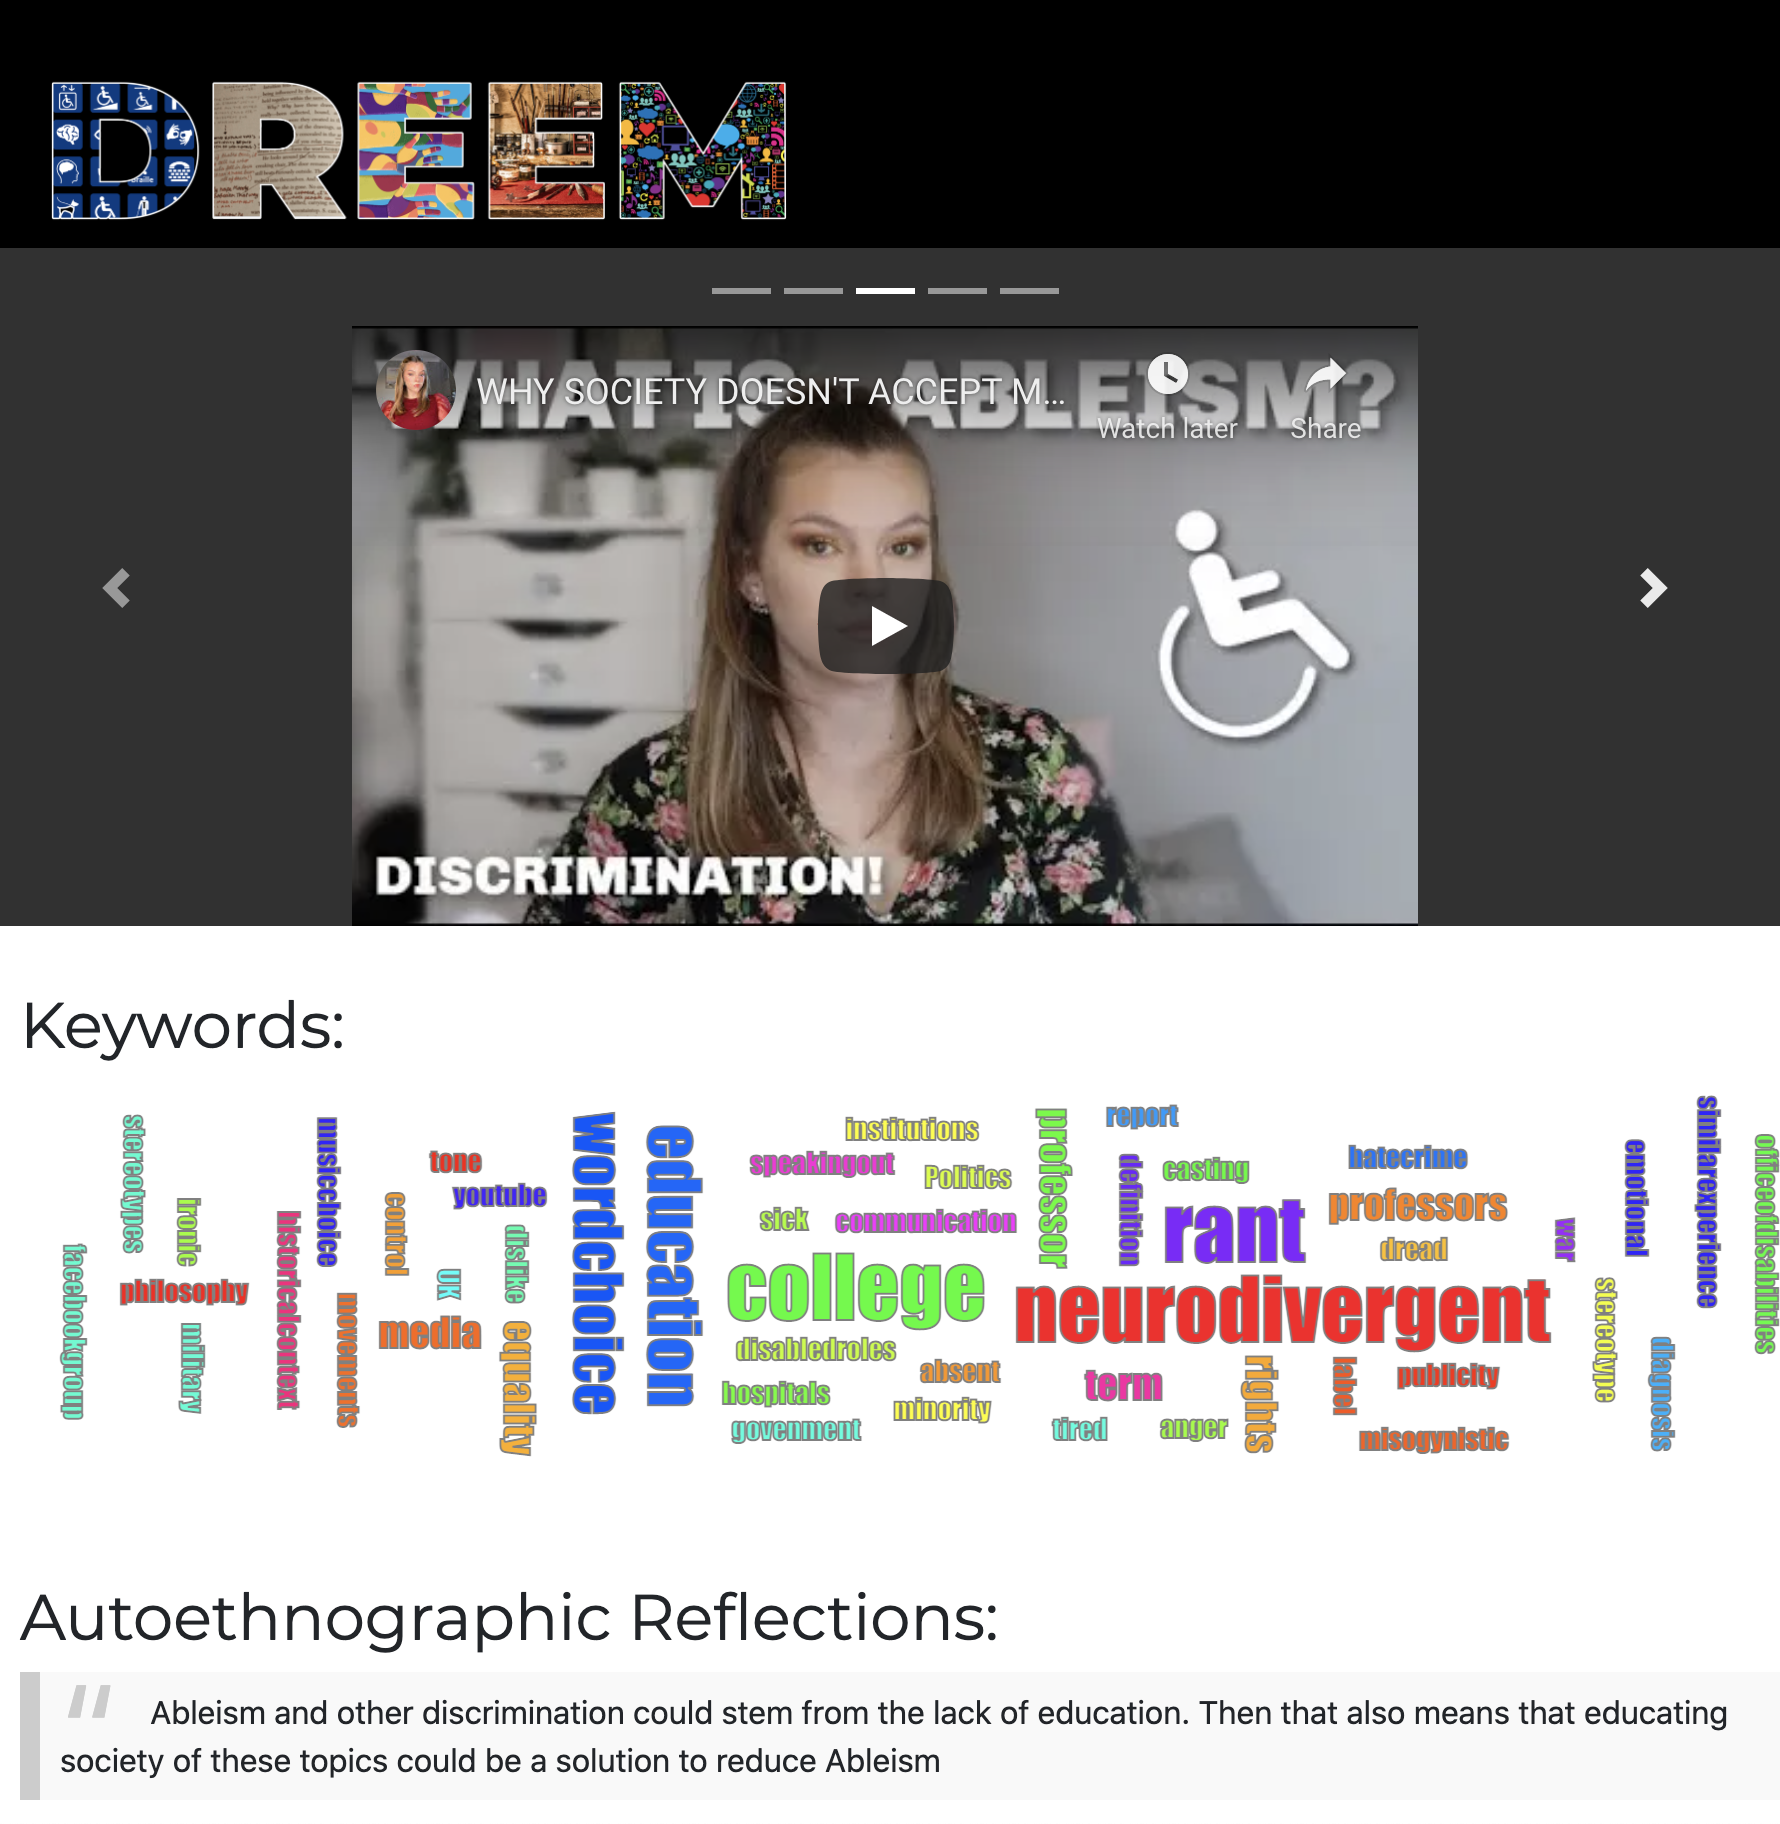
\includegraphics[width=\linewidth]{Figures/Reviewer.png}
    \Description{The review tool uses a carousel to flip through the various media sources quickly and see relevant close readings below, sorted by time or location. Under the carousel is a word cloud of the keywords to visualize the qualitative themes. There is a specific area for direct quotes that highlight the autoethnographic reflections}
    \caption{A screenshot of the DREEM review tool. Users can upload their close readings to analyze what they've collected all in one place.}
    \label{fig:reviewer}
\end{figure}
While there are many compelling software-based annotation tools and qualitative visualizations used by scholars in Digital Humanities \cite{janickeCloseDistantReading2015}, we found no easy way to experience our dense reflections at a higher level. While constructing our case studies, we struggled with how to present DREEM findings for higher-level reflections, so we decided to create a website that was highly effective in assisting with our analysis, shown in Figure \ref{fig:reviewer}. The website allows researchers to import data from the DREEM Google Form related to a particular topic. The website dynamically loads media sources including \textit{TikToks}, \textit{YouTube} videos, website previews, and podcasts into a carousel that the researcher can flip through. The table at the bottom of the page only shows close readings that correspond to the active media source in the carousel. A word-cloud of keywords is automatically generated and the autoethnographic reflections are highlighted in block quotes. The current version of the tool is available at: \url{https://tinyurl.com/DREEMReviewTool} and we plan to make updates to the <anonymous> public \textit{GitHub} repository. 

\subsection{How to Present DREEM Findings}
DREEM findings can be presented as their own findings, or as step within a larger body of work. In each case the presentation of the work will look slightly different. This method generates research questions, so it is likely that the findings will become a part of the larger body. In the case that DREEM is presented as the primary finding, the outcome may look similar to a traditional close reading that focuses on a particular topic and discusses multiple sources. \cite{cullenBetterWorldExamples2018} and \cite{mingusReflectingFridaKahlo2010} are two good, and very different, examples of close readings.

We encourage researchers to share important elements that are specific to the DREEM process such as links to all media analyzed (regardless of if it is discussed in the body of text), keywords and their frequency, and a thematic analysis of the individual close readings and/or reflections. 

\subsection{DREEMing as a Team}
DREEMing can be done on your own or as a team. If you plan to work as a team, we offer some insights based on our experiences.

We found that DREEMing has the potential as an effective way for undergraduate research assistants and assistive technology newcomers to become acquainted with people with disabilities. DREEMing as a team offers the ability to discuss and build on each other's work. As has been discussed in other literature, teaching accessibility concepts to undergraduates continues to be a challenge \cite{shinoharaDesignSocialAccessibility2020}. We offer this as one framework for learning towards that goal. 

It is not required for multiple team members to do close readings of the same media. However, doing so can offer insights from multiple perspectives. We found that comparing each other's notes led to fruitful conversations about the researcher's individual experiences and insights that might have been missed if everyone was working independently. We recommend, leaving time in your research process to read each other's close readings and journals and meet to discuss them. Teams should work together to find a logging process that works for everyone. Expectations for quality and length of passages should be set and continually talked about. 

\section{Final Thoughts and Conclusion} \label{Discussion}
To conclude, we will leave the reader with some final thoughts on the opportunities and challenges presented with DREEM, future directions, and summary of this work.

\subsection{Opportunities}
DREEM has become increasingly relevant in the wake of COVID-19. It can be challenging to include people with disabilities for participatory and community-based work generally \cite{wardReflectionsParticipatoryAction2001}, but there is a specific added risk during a global pandemic. In addition to general guidelines that limit in-person contact, populations of people with disabilities often have medical needs that place them at higher risk from the COVID19 virus \cite{armitageCOVID19ResponseMust2020}. In light of quarantine, designers are employing creative methodologies to carry out remote design work that is usually done in situ \cite{whiteLearningCOVID19Design2020} (e.g., using games to educate the public about COVID19 and collect data \cite{lopezherna;ndezHealthcareGamificationSerious2020}). Many of these technologies are not accessible to people with disabilities \cite{annaswamyTelemedicineBarriersChallenges2020}. DREEM allows researchers to safely conduct preliminary research in preparation for participatory work when in-person protocols are safe after ubiquitous vaccination. 

DREEM surfaces and features existing work and labor of disabled people. The validity of research can be more rigorous if the source of inspiration is surfaced and credit is given where it is due. DREEM extends participatory design and community-based research from being inclusive on \textit{how} something should be made to \textit{what} should be made in the first place.

\subsection{Challenges \& Limitations}
This method requires access to content created and posted online. Content creators with particular disabilities are relatively few on some mediums due to accessibility issues. Memes and GIFs for instance are often posted without alt text \cite{gleasonMakingGIFsAccessible2020}, so the participation of screen reader users with Memes and GIFs may be lower. Related, different social media platforms have their own affordances and norms as discussed in the previous section. Therefore, investigating multiple platforms will help increase the diversity of the findings using DREEM.

Researchers must be careful not to over generalize as not every disabled individual will be represented by those who are creating content online (i.e., a disabled individual who does not have access to creating certain media or has no desire to create content on social media may have a very different experience than someone who does have access and a desire to create and post content.) %The verification step can help to neutralize this issue, but requires that you verify with a different subset of the population, which can be tricky to know. 

Finally, the challenge of training individuals to recognize and flag ableism and ableist content is ongoing. We have tried to mitigate this with our trainings and suggestions in this paper, but recognize this is a thorny issue that will need continual appraisal.

\subsection{Future Work}
In this paper, we present several case studies that demonstrate DREEM. However, the research agenda created by the findings of each case study have yet to be enacted. Application of this method to longer term projects is needed. The research team intends to follow up on the case studies presented here as their own research projects. We chose to conduct the survey in Section \ref{survey} as our findings developed because we saw the change in the undergraduate researchers language and comfort around topics of disability. 
In the future it would be worthwhile to conduct the survey twice as both a pre and post survey. Our work with DREEM has primarily considered videos and text passages. More work should be done to DREEM with visual art and audio. We are excited to see what others come up with when using DREEM. 

\subsection{Conclusion}
In this paper, we propose DREEM, a 4-step nascent method for using close readings of media posted by people with disabilities to build empathy and authentic research agendas prior to participatory work. Our primary contributions include materials for utilizing DREEM, including trainings, data logging templates, and a tool for visualizing close readings. We found that actively engaging with media made by people with disabilities is an opportunity for new researchers to learn about these communities and working with disabled people. The potential benefits of continuing this line of work include shared labor, authentic research problems, increased visibility of disability communities, and healthier partnerships with communities of people with disabilities. 

%We explore three research questions: %\begin{enumerate}[label=RQ\arabic*:]
%\item \textit{What can assistive technology researchers and designers utilize media made by disabled people in their work? (DREEM)}
%\item \textit{What types of insights does DREEM offer?} %through employing it in case studies?}
%\item \textit{How can scholars adopt DREEMing efficiently?}
%\end{enumerate} 
%<<outcomes >>

%Our contributions are...
%<<access tools by...>>



%\balance
%\begin{acks}

%\end{acks}